% =====================================================================
%  ch03c.tex —— 第 3 章 Chern–Simons 微扰理论 · §3.3 + 小结 + 章末评注
%  原书 p.117–p.125（PDF 137–145）  译者：Lead（接手）
% =====================================================================

% [原文 p.117]
\section{由 Chern--Simons 微扰理论构造拓扑不变量}

\takeaway{本节先看 $G=U(1)$ 的情形：配分函数是二次与一次形式之和的 Gauss 型积分，其核由 Green 形式的积分给出，正是环绕数的积分表示。对 $SU(2)$ 情形，$k\to\infty$ 的渐近展开由平坦联络附近的 Feynman 图给出；Axelrod--Singer 用 Green 形式的积分（两条 2 圈图 $I_{\Gamma_1},I_{\Gamma_2}$）加上引力 Chern--Simons 项 $(1/4)CS_{\mathrm{grav}}(g,s)$，构造出不依赖 Riemann 度量的三维流形拓扑不变量。}

先从 $G=U(1)$ 的情形开始。设 $L=K_1\cup K_2$ 为 $\R^{3}$ 内由两个分支构成的链环。设 $A$ 为 $\R^{3}$ 上 $U(1)$ 联络全体的空间。它可以与 $\R^{3}$ 上取值于 $\R$ 的一次微分形式的空间等同。这种情形下，对应于表示 Chern--Simons 泛函配分函数的式 (2.41) 的式子为
\begin{equation}
  Z_k=\int_{\mathcal{A}}\exp\Bigl(\frac{\sqrt{-1}k}{4\pi}\int_{\R^{3}}A\wedge dA
  +\sqrt{-1}\int_{K_1}A+\sqrt{-1}\int_{K_2}A\Bigr)\,\mathcal{D}A \tag{3.25}
\end{equation}
Chern--Simons 泛函可以看作：把由 $A\mapsto A\wedge dA$ 表示的联络空间上的二次形式，在保持规范不变性的前提下推广到非交换的情形。像式 (3.25) 这样、关于二次形式与一次形式之和的指数函数的路径积分，在 Feynman 路径积分中是理解得比较清楚的一类，可用 Gauss 积分的反复表示。

先用有限维积分的类比来说明。对非退化二次形式
\[
  Q(x_1,\dots,x_n)=\frac{1}{2}\sum_{ij}\lambda_{ij}x_ix_j,
\]
考虑积分
\[
  \int_{\R^{n}}e^{\sqrt{-1}\bigl(Q(x_1,\dots,x_n)+\sum_{j=1}^{n}\mu_jx_j\bigr)}\,dx_1\cdots dx_n .
\]
通过配方，上述积分除常数倍外可化为
\[
  e^{-\sqrt{-1}\frac{1}{2}\sum_{ij}\lambda^{ij}\mu_i\mu_j}
\]
的形状。这里 $(\lambda^{ij})$ 是 $(\lambda_{ij})$ 的逆矩阵。

回到无限维积分 $Z_k$ 的情形。其实这种情形也可以用微分算子 $d$ 的逆算子来描写。逆算子是
\[
  (\tilde L\varphi)(x)=\int_{y\in\R^{3}}L(x,y)\wedge\varphi(y)
\]

% [原文 p.118]
形状的积分算子，积分核 $L$ 称为 \textbf{Green 形式}。在 $\R^{3}$ 的情形，Green 形式 $L$ 如下表示。对向量 $x\in\R^{3}\setminus\{0\}$，令
\begin{equation}
  w(x)=\frac{x_1\,dx_2\wedge dx_3+x_2\,dx_3\wedge dx_1+x_3\,dx_1\wedge dx_2}{4\pi\|x\|^{3}} . \tag{3.26}
\end{equation}
它给出按 $\int_{S^{2}}w(x)=1$ 归一化的球面体积元素。用这个 $w$，Green 形式表为
\[
  L(x,y)=w(x-y).
\]
积分 $Z_k$ 的主要部分中出现
\[
  \int_{x\in K_1,\ y\in K_2}w(x-y).
\]
这个积分就是 Gauss 求得的环绕数的积分表示。

其次讨论 $SU(2)$ Chern--Simons 理论配分函数在 $k\to\infty$ 时的渐近行为。正如 3.2 节所述，渐近展开主项的贡献被认为来自 Chern--Simons 泛函的临界点，即平坦联络。这里也假定平坦联络 $\alpha$ 满足 $H^{*}(M,\mathfrak{g}_\alpha)=0$。

先在有限维情形介绍用 Feynman 图表示积分
\begin{equation}
  Z_k=\int_{\R^{n}}e^{\sqrt{-1}kf(x_1,\dots,x_n)}\,dx_1\cdots dx_n \tag{3.27}
\end{equation}
在 $k\to\infty$ 时渐近展开高次项的方法。考虑 (3.27) 中 $f$ 可用非退化二次形式 $Q$ 表为
\[
  f(x_1,\dots,x_n)=Q(x_1,\dots,x_n)+\sum_{ijk}\lambda_{ijk}x_ix_jx_k
\]
的情形。通过变量替换，可把 $Z_k$ 表为
\[
  Z_k=k^{n/2}\int_{\R^{n}}e^{\sqrt{-1}\bigl(Q(x_1,\dots,x_n)+\sum_{m=0}^{\infty}\frac{1}{m!}\bigl(\sum_{ijk}\lambda_{ijk}x_ix_jx_k\bigr)^{m}\bigr)}
  \,dx_1\cdots dx_n .
\]
为求积分 $Z_k$ 在 $k\to\infty$ 时的渐近展开，

% [原文 p.119]
计算积分
\begin{equation}
  \int_{\R^{n}}e^{\sqrt{-1}Q(x_1,\dots,x_n)}
  \Bigl(\sum_{ijk}\lambda_{ijk}x_ix_jx_k\Bigr)^{m}\,dx_1\cdots dx_n . \tag{3.28}
\end{equation}
引入变量 $J_1,\dots,J_n$，利用微分算子
\[
  D_j=\frac{1}{\sqrt{-1}}\frac{\partial}{\partial J_j},
\]
可把它表为
\[
  \Bigl[\Bigl(\sum_{ijk}\lambda_{ijk}D_iD_jD_k\Bigr)^{m}
  \int_{\R^{n}}e^{\sqrt{-1}\bigl(Q(x_1,\dots,x_n)+\sum_{k}J_kx_k\bigr)}
  \,dx_1\cdots dx_n\Bigr]_{J=0}.
\]
因此用配方可知，积分 (3.28) 除适当常数倍外等于
\[
  \Bigl[\Bigl(\sum_{ijk}\lambda_{ijk}D_iD_jD_k\Bigr)^{m}
  e^{-\sqrt{-1}\frac{1}{2}\sum_{ij}\lambda^{ij}J_iJ_j}\Bigr]_{J=0}.
\]
它是 $\lambda^{ij}$ 与 $\lambda_{ijk}$ 的多项式，且仅在 $m$ 为偶数时不为 $0$。$m=2$ 时具体地表为
\[
  \sum_{ijk\,i'j'k'}\lambda_{ijk}\lambda_{i'j'k'}\lambda^{ii'}\lambda^{jj'}\lambda^{kk'}
\]
形状的项，与
\[
  \sum_{ijk\,i'j'k'}\lambda_{ijk}\lambda_{i'j'k'}\lambda^{ij}\lambda^{kk'}\lambda^{i'j'}
\]
形状的项之和。把它们分别如图 3.4 用一个顶点处汇集 3 条边的图表示。这样的图称为 2 圈的 \textbf{Feynman 图}。一般地，对偶数 $m$，渐近展开中出现的项可用有 $m$ 个顶点、每个顶点周围汇集 3 条边的图来描述。它们称为 $m$ 圈的 Feynman 图。

把这样的手法形式地应用于 Chern--Simons 泛函的配分函数

% [原文 p.120]
\begin{figure}[htbp]
  \centering
  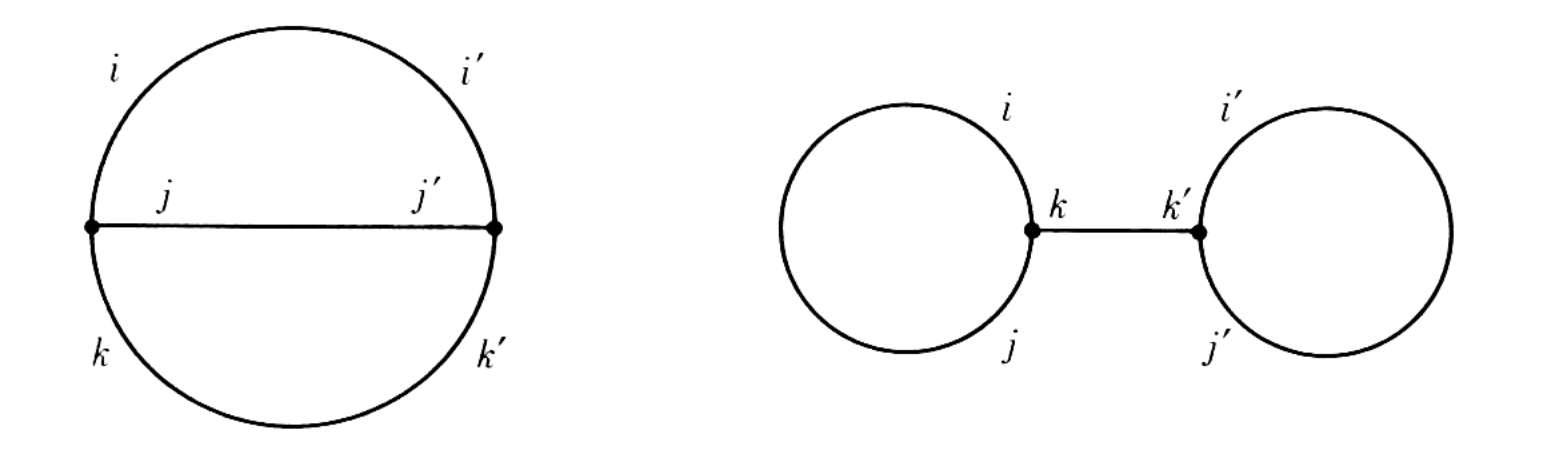
\includegraphics[width=0.38\textwidth]{figures/fig3.4.png}
  \figtitle{3.4}{2 圈的 Feynman 图（原书 p.120）}
\end{figure}

\[
  Z_k(M)=\int_{\mathcal{A}_M}\exp\bigl(2\pi\sqrt{-1}k\,CS(A)\bigr)\,\mathcal{D}A
\]
时，除无限维空间 $\mathcal{A}_M$ 上测度的问题之外，还有若干困难之处。Chern--Simons 泛函的临界点是平坦联络。这里要考察 $Z_k$ 在 $k\to\infty$ 时的渐近行为，但正如 3.2 节所述，Chern--Simons 泛函局部地在规范变换下不变，Hessian 沿规范轨道退化。

再次回到有限维积分，说明这种状况下的手法。取 $G$ 为 $l$ 维 Lie 群，设 $G$ 作为 $\R^{n}$ 的等距变换作用，且
\[
  f(x_1,\dots,x_n)=Q(x_1,\dots,x_n)+\sum_{ijk}\lambda_{ijk}x_ix_jx_k
\]
在 $G$ 的作用下不变。又设存在光滑函数 $F\colon\R^{n}\to\R$，$F$ 在每个 $G$ 轨道上恰有一个零点。关注满足 $F(x)=0$ 的 $x\in\R^{n}$ 处的 $G$ 轨道 $Gx$。定义映射 $\psi\colon G\to\R$ 为 $\psi(g)=F(gx)$，把 $\psi$ 在 $G$ 的单位元处的 Jacobi 矩阵记作 $J(x)$。行列式 $\det J(x)$ 表示 $G$ 轨道 $Gx$ 的体积元素与 Lie 群 $G$ 的体积元素之比。积分 (3.27) 照原样会把同一个积分沿 $G$ 轨道无限重复计算，故取出本质部分后为
\begin{equation}
  \int_{\R^{n}}e^{\sqrt{-1}kf(x_1,\dots,x_n)}
  \delta(F(x))\det J(x)\,dx_1\cdots dx_n . \tag{3.29}
\end{equation}
这里 $\delta$ 是 Dirac 的 $\delta$ 函数。对这一部分用 Fourier 变换

% [原文 p.121]
表为
\[
  \delta(F(x))=\frac{1}{(2\pi)^{l}}\int_{\R^{l}}e^{\sqrt{-1}\sum_{i=1}^{l}F_i(x)\varphi_i}
  \,d\varphi_1\cdots d\varphi_l,
\]
把 $\varphi_1,\dots,\varphi_l$ 作为新的积分变量加入，就能把 $\delta$ 函数的部分并入作用量。Jacobi 行列式的部分用下列方法同样可以并入作用量。引入称为 Grassmann 变量的变量组 $\{c_i\},\{\bar c_i\}$（$1\le i\le l$）。它们彼此反交换，满足
\[
  c_ic_j+c_jc_i=0,\qquad \bar c_i\bar c_j+\bar c_j\bar c_i=0,\qquad
  \bar c_ic_j=c_j\bar c_i,\qquad 1\le i,j\le l .
\]
行列式 $\det J$ 除常数倍外表为
\[
  \int e^{\sqrt{-1}\operatorname{tr}J(x)\,\bar c_1c_1\cdots\bar c_l c_l}
  \,d\bar c_1\,dc_1\cdots d\bar c_l\,dc_l .
\]
这样，通过加入变量 $\varphi_1,\dots,\varphi_l$ 与 Grassmann 变量 $\{c_i\},\{\bar c_i\}$（$1\le i\le l$），可以把积分 (3.29) 被积函数的部分全部放到 $e$ 的指数上，并入作用量。关于 Grassmann 变量，请参阅例如文献 [3] 等。

以上虽只是有限维的类比，但在 Chern--Simons 泛函的配分函数中，为消除沿规范轨道的退化问题，也要在平坦联络 $\alpha$ 附近，把积分限制在满足 $d_\alpha^{*}A=0$ 的 $A$ 上。这对应于上面的 $F(x)=0$，称为\textbf{规范固定}（gauge fixing）。为此再引入费米子场 $c,\bar c$ 与玻色子场 $\varphi$。这里所用的手法称为 BRS 形式。

Axelrod--Singer [18] 以上述预备性考察为基础，构造了用 Green 形式积分表示的三维流形拓扑不变量。设 $M$ 为紧的、带定向、无边界的三维流形。取 $M$ 上主 $SU(2)$ 丛的平坦联络 $\alpha$，假定 $\alpha$ 满足 $H^{*}(M,\mathfrak{g}_\alpha)=0$。固定 $M$ 的 Riemann 度量，考虑 $d_{(\alpha,\alpha)}^{\mp1}$ 的积分核
\[
  L\in\Omega^{2}(M\times M;\mathfrak{g}\otimes\mathfrak{g}).
\]
这里 $\Delta_\alpha$ 是 3.2 节的 Laplace 算子 $\Delta_\alpha^{0},\dots,\Delta_\alpha^{3}$ 的直和。取 $SU(2)$ 的 Lie 代数 $\mathfrak{g}$ 的正规正交基 $\{I_a\}$（$a=1,2,3$），

% [原文 p.122]
表为
\[
  L=\sum L_{ab}(x,y)\,I_a\wedge I_b .
\]
$L$ 是 Green 形式；把 $M\times M$ 上以局部系 $\mathfrak{g}_\alpha\otimes\mathfrak{g}_\alpha$ 为系数的 de Rham 复形的共变微分记作 $d_{(\alpha,\alpha)}$，则
\begin{equation}
  d_{(\alpha,\alpha)}L_{ab}(x,y)=-\delta_{ab}\,\delta(x,y) \tag{3.30}
\end{equation}
成立。这里 $\delta(x,y)$（$(x,y)\in M\times M$）是表示对角集合 $\Delta\subset M\times M$ 的 Poincaré 对偶的 3 次微分形式，对 $M\times M$ 上的 3 次微分形式 $\psi(x,y)$ 满足
\[
  \int_{M\times M}\delta(x,y)\psi(x,y)=\int_{M}\psi(x,x).
\]
又，
\[
  L_{ab}(x,y)=-L_{ba}(y,x)
\]
成立。

把 Lie 代数 $\mathfrak{g}$ 的结构常数记作 $\{\gamma_{abc}\}$。对应于图 3.4 所示的 2 圈 Feynman 图，令
\begin{align*}
  I_{\Gamma_1}(M,\alpha)
  &=-\frac{1}{8}\sum\int_{M\times M\setminus\Delta}
  \gamma_{a_1b_1c_1}\gamma_{a_2b_2c_2}\notag\\
  &\qquad\times L_{a_1c_1}(x_1,x_1)\wedge L_{a_2c_2}(x_2,x_2)\wedge L_{b_1b_2}(x_1,x_2),\\
  I_{\Gamma_2}(M,\alpha)
  &=\frac{1}{12}\sum\int_{M\times M\setminus\Delta}
  \gamma_{a_1b_1c_1}\gamma_{a_2b_2c_2}\notag\\
  &\qquad\times L_{a_1a_2}(x_1,x_2)\wedge L_{c_1c_2}(x_1,x_2)\wedge L_{b_1b_2}(x_1,x_2).
\end{align*}
这里不作详细说明，但 $L_{a_1c_1}(x_1,x_1)$ 等是对角集合处除去 Green 形式奇异性项来定义的。由 Axelrod--Singer [18]，证明了下列定理。

\begin{theorem}{3.5}
  （Axelrod--Singer）在关于三维流形 $M$ 及其上 $SU(2)$ 平坦联络 $\alpha$ 的上述假设之下，
  \[
    I_{\Gamma_1}(M,\alpha)+I_{\Gamma_2}(M,\alpha)-\frac{1}{4}CS_{\mathrm{grav}}(g,s)
  \]
  是不依赖于 Riemann 度量的 $M$ 的拓扑不变量。
\end{theorem}

上述定理中的 $CS_{\mathrm{grav}}(g,s)$，是关于 $M$ 的切丛上由 $M$ 的 Riemann 度

% [原文 p.123]
量自然定出的 Levi--Civita 联络的 Chern--Simons 泛函的值。它由 $M$ 的切丛的平凡化即 $M$ 的 framing $s$ 给定。以下叙述定理证明的概略。

为证明定理所述之量不依赖 $M$ 的 Riemann 度量，考虑 $M$ 的 Riemann 度量的单参数族 $\{g_t\}$。与之对应得到 Green 形式的单参数族 $L_t$。把关于参数 $t$ 的微分记作 $\nabla$，则由式 (3.30)，$d_{(\alpha,\alpha)}L$ 不依赖 $M$ 的 Riemann 度量，故得
\[
  d_{(\alpha,\alpha)}\nabla L_t=0 .
\]
因此，由假设 $H^{*}(M,\mathfrak{g}_\alpha)=0$，存在取值于 $\mathfrak{g}\otimes\mathfrak{g}$ 的 $M\times M$ 上一次微分形式 $B$，满足
\begin{equation}
  \nabla L_t=d_{(\alpha,\alpha)}B . \tag{3.31}
\end{equation}
这里把 $L_t$ 略记为 $L$。

其次如下构造流形 $\Conf_2(M)=M\times M\setminus\Delta$ 的紧化。考虑 $M\times M$ 沿 $\Delta$ 的实流形意义下的爆破 $\pi\colon\widehat{M\times M}\to M\times M$。$\pi^{-1}(\Delta)$ 与由 $M$ 的切丛的子丛、即切向量长度全为 1 者构成的 $SM$ 等同。$SM$ 是 $M$ 上的 $S^{2}$ 丛。$\widehat{M\times M}$ 是带边界的紧流形，其内点集合与 $M\times M\setminus\Delta$ 等同，边界与 $SM$ 等同。作为 $\Conf_2(M)$ 的紧化 $\overline{\Conf_2(M)}$，采用这个 $\widehat{M\times M}$。积分 $I_{\Gamma_1},I_{\Gamma_2}$ 都可以看作 $\overline{\Conf_2(M)}$ 上的积分，且可证明积分取有限值。用式 (3.31)、式 (3.30) 以及 Stokes 定理，计算 $\nabla I_{\Gamma_j}$（$j=1,2$）。关于 $\nabla I_{\Gamma_1}$，它表为 $\overline{\Conf_2(M)}$ 上的积分
\begin{align*}
  &\frac{1}{8}\int_{\overline{\Conf_2(M)}}\sum \gamma_{a_1b_1c_1}\gamma_{a_2b_2c_2}
  B_{a_1c_1}(x_1,x_1)L_{a_2c_2}(x_2,x_2)\delta_{b_1b_2}\delta(x_1,x_2)\\
  &\quad+\frac{1}{8}\int_{\overline{\Conf_2(M)}}\sum \gamma_{a_1b_1c_1}\gamma_{a_2b_2c_2}
  L_{a_1c_1}(x_1,x_1)B_{a_2c_2}(x_2,x_2)\delta_{b_1b_2}\delta(x_1,x_2)
\end{align*}
与 $\partial\overline{\Conf_2(M)}$ 上的积分之和。这里只把 $\overline{\Conf_2(M)}$ 上积分的项合并，得
\begin{equation}
  \frac{1}{4}\int_{M}\sum\gamma_{acd}\gamma_{aef}\,B_{cd}(x,x)L_{ef}(x,x) \tag{3.32}
\end{equation}
同样地，从 $I_{\Gamma_2}$ 得到 $\overline{\Conf_2(M)}$ 上积分的项
\begin{equation}
  \frac{1}{4}\int_{M}\sum\bigl(\gamma_{ace}\gamma_{afd}-\gamma_{acf}\gamma_{aed}\bigr)
  B_{cd}(x,x)L_{ef}(x,x) \tag{3.33}
\end{equation}
这里和取遍 $a,c,d,e,f$。对式 (3.32) 与式 (3.33) 用图 3.5 所示的 Lie 代数的 Jacobi 等式与 Lie 括号的反对称性，可知这些和为零。进一步（这里不详述），可以证明从 $\partial\overline{\Conf_2(M)}$ 上的积分出现 $CS_{\mathrm{grav}}$ 的项。

% [原文 p.124]
\begin{figure}[htbp]
  \centering
  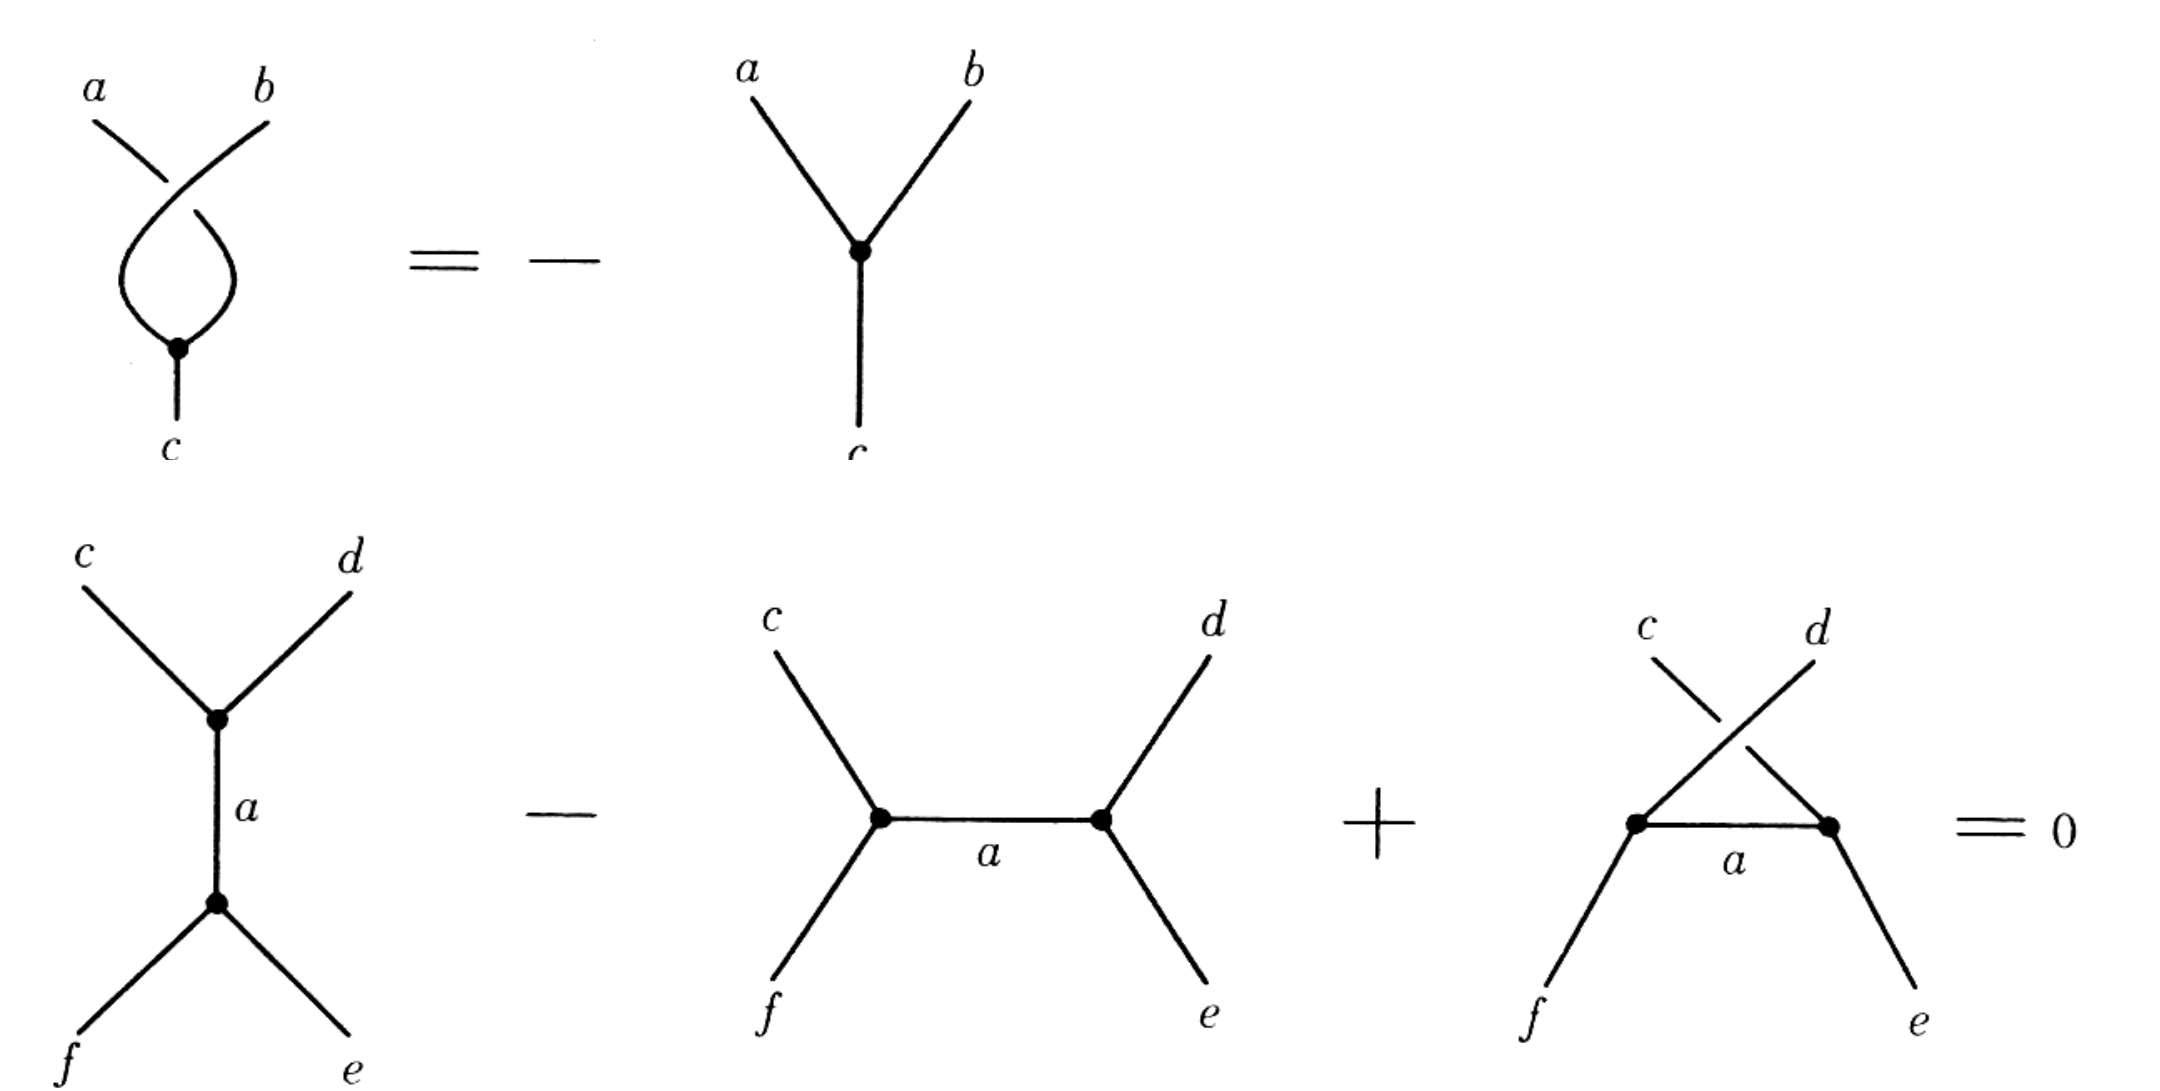
\includegraphics[width=0.84\textwidth]{figures/fig3.5.png}
  \figtitle{3.5}{上：Lie 括号的反对称性；下：Jacobi 等式的图表示（原书 p.123）}
\end{figure}

% [原文 p.125]
\section*{小结}
\addcontentsline{toc}{section}{小结}
\markright{小结}

\begin{itemize}[leftmargin=2em,itemsep=2pt]
\item 3.1 定义了纽结的 Vassiliev 不变量，并给出 Kontsevich 的迭代积分表示。
\item 3.2 在 Chern--Simons 泛函的临界点即平坦联络处，计算 Hessian 的正规化行列式，说明了 Ray--Singer 挠率的出现。
\item 3.3 描述了由 Chern--Simons 微扰理论导出的三维流形拓扑不变量。
\end{itemize}

\chapterreview{第 3 章把前两章的「不变量」推进到「微扰展开」这一层次，可以看作全书方法论上的收束。

\textbf{全章地位。}第 1 章给出共形块与 KZ 方程，第 2 章用其和乐构造辫群表示与 Witten 不变量；本章则换一条路线：不追求严格定义路径积分，而是把配分函数在临界点附近形式地展开，用 Feynman 图逐阶提取有限量。Vassiliev 不变量与 Kontsevich 积分提供了「纽结侧」的通用框架，Axelrod--Singer 的 Green 形式积分提供了「三维流形侧」的框架，二者都以「有限阶/有限圈」的截断把无限维问题化为有限维计算。

\textbf{知识脉络。}§3.1 从结空间 $\cM\setminus\Sigma$ 的 上同调 出发，把有限阶不变量化为弦图模去 4 项关系式后的对偶空间 $\cA_m^{*}$；Kontsevich 定理（定理 3.3）说明这个对偶空间恰由积分给出。§3.2 处理 Chern--Simons 泛函临界点的 Hessian，Ray--Singer 挠率作为正规化行列式出现。§3.3 把上述两条线索合到三维流形：$U(1)$ 情形退化为 Gauss 型积分与环绕数；$SU(2)$ 情形则要处理规范轨道退化，用规范固定（BRS 形式）把 Jacobi 行列式并入作用量。

\textbf{核心结论。}(3.25) 表明 $U(1)$ 配分函数的核心是 Green 形式的积分，即环绕数；(3.27)–(3.28) 给出 $k\to\infty$ 渐近展开的有限维模型，其主项来自临界点、高次项由 Feynman 图给出；(3.30)–(3.33) 与定理 3.5 表明，两条 2 圈图的 Green 形式积分加上 $(1/4)CS_{\mathrm{grav}}$ 后，对 Riemann 度量不变。

\textbf{辨析与提醒。}其一，本章所有「路径积分」都是形式的，作者也反复声明测度未严格定义；读时要把每个积分理解为「在有限维类比下被证明了的展开式」。其二，(3.17) 的指数是 $-\mu(K)+1$，容易误读为 $-\mu(K)-1$。其三，$I_{\Gamma_1},I_{\Gamma_2}$ 中对角项 $L_{aa}(x,x)$ 通过「除去奇异性项」定义，这一步在原文中是略去的技术要点，不能按普通 Green 形式代入。

\textbf{评注。}本章的证明只到「概略」程度，Axelrod--Singer 定理的完整验证（尤其是 $\partial\overline{\Conf_2(M)}$ 上积分的边界项）超出了本书篇幅。读者若要与现代文献对照，可注意两点：现行文献多用「构形空间上的 Fulton--MacPherson 紧化」代替此处的爆破叙述；$CS_{\mathrm{grav}}$ 项与 framing 的关系，在 Reshetikhin--Turaev 的量子群框架下有更初等的对应。}

% [Tutor Note: (3.25) 中 $k/4\pi$ 的归一化与第 2 章 (2.41) 一致；$\int_{K_i}A$ 两项是 Wilson 线在 $U(1)$ 情形的线性项，正是它们把链环信息带进配分函数。若把 $k$ 换成 $1/\hbar$ 并与 (3.27) 对照，可以看出「大 $k$ 渐近」与「半经典极限」是同一件事。]

% [Tutor Note: (3.26) 的 $w(x)$ 是 $\R^{3}$ 中球面 $S^{2}$ 的体积元素在 $\R^{3}\setminus\{0\}$ 上的拉回，$\int_{S^{2}}w=1$ 的归一化决定了 Green 形式 $L(x,y)=w(x-y)$ 与环绕数积分 $\int\!\!\int w(x-y)$ 的符号约定；符号一旦改，整个 $I_{\Gamma}$ 的符号随之改变。]

% [Tutor Note: (3.28) 中 $m=2$ 的两项分别对应两种把 4 个指标两两配对的缩并方式（$\lambda^{ii'}\lambda^{jj'}\lambda^{kk'}$ 与 $\lambda^{ij}\lambda^{kk'}\lambda^{i'j'}$），在图上就是 2 圈 Feynman 图的两种连边方式。]

% [Tutor Note: 定理 3.5 中的 $(1/4)CS_{\mathrm{grav}}(g,s)$ 是「引力 Chern--Simons 项」，依赖切丛的 framing $s$ 的选取；它补偿了 $I_{\Gamma_1}+I_{\Gamma_2}$ 在改变 framing 时的变化，因此最终结果才可能不依赖度量的选取。作者在正文中略去了这一项的构造，只说明它出现。]

% [Tutor Note: (3.32) 与 (3.33) 都含有 $\sum_a\gamma_{acd}\gamma_{aef}$ 型的结构常数缩并；用 Jacobi 等式 $\gamma_{ace}\gamma_{bfd}$ 型恒等式与反对称性把它们消去，是证明「$\nabla I_{\Gamma}$ 只有边界项」的关键一步，也是全书唯一一处真正使用 Lie 代数 Jacobi 等式的计算。]

% CHUNK ch03c DONE
